\input{Configuraciones/paquetes}

%--------------------------

\begin{document}
 \thispagestyle{empty} 
    \begin{tabular}{p{15.5cm}}
    \begin{tabbing}
    \textbf{Universidad del Valle de Guatemala} \\\\
   \textbf{Estudiantes:} Rudik Rompich, Alejandro García Aguirre, Lisandro Toruño\\

    \end{tabbing}
    \begin{center}
        Teoría electromagnética 1 - Catedrático: Eduardo Álvarez\\
        \today
    \end{center}\\
    \hline
    \\
    \end{tabular} 
    \vspace*{0.3cm} 
    \begin{center} 
    {\Large \bf  Simulación
} 
        \vspace{2mm}
    \end{center}
    \vspace{0.4cm}
%--------------------------

\begin{problema}
    Suponga que al rod-cutting problem agregamos un límite piezas que se pueden vender o cortar para cada posible tamaño. Es decir que, para $0<i \leq n, l_{i} \in \mathbf{N}$ es el número máximo de piezas de tamaño $i$ que podemos usar en la solución. Demuestre que con esta nueva restricción el problema ya no exhibe una subestructura óptima. Hint: ¿qué característica de los subproblemas se evaluó para determinar la ausencia de subestructura óptima en el unweighted longest simple path problem?
    \begin{sol}
        Para demostrar que el problema modificado del corte de varillas con límites en la cantidad de piezas ya no exhibe una subestructura óptima, consideremos la característica que se evaluó en el unweighted longest simple path problem: la subestructura óptima se rompe debido a que el óptimo global no se construye necesariamente a partir de soluciones óptimas a subproblemas.\bigbreak

        Tenemos que una subestructura óptima si una solución óptima al problema contiene soluciones óptimas a sus subproblemas Ahora, en el problema modificado, para cada tamaño de varilla $i$, tenemos un límite $l_i$ en la cantidad de piezas que se pueden vender o cortar.\bigbreak

        Para responder esta pregunta, se propone un contraejemplo:\bigbreak
        
        Supongamos que tenemos una varilla de longitud $n = 4$ y los precios son $p = [1, 4, 4, 6]$ (donde $p_i$ es el precio de una varilla de longitud $i$). Además, los límites para cada tamaño de varilla son $l = [1, 1, 2, 1]$. 
        \begin{itemize}
            \item La solución óptima al problema original (sin límites) sería cortar la varilla en dos piezas de longitud 2, con un ingreso total de 8. En este caso, los subproblemas también tienen soluciones óptimas: no cortar las varillas de longitud 2.

            \item Sin embargo, con los límites introducidos, la solución óptima cambia. Ahora, no podemos cortar la varilla en dos piezas de longitud 2 porque el límite $l_2 = 1$. En cambio, la solución óptima es cortar la varilla en una pieza de longitud 1 y otra de longitud 3, con un ingreso total de 5. Aquí, la solución óptima para el subproblema de longitud 1 (no cortarla) no se combina con la solución óptima para el subproblema de longitud 3 (no cortarla) para formar la solución óptima global.
        \end{itemize}

        Este ejemplo muestra que, con la restricción adicional de límites en la cantidad de piezas, el problema modificado del corte de varillas ya no exhibe una subestructura óptima.
        
    \end{sol}

\end{problema}

\begin{problema}
    Volvamos al rod-cutting problem original. Resulta que no tenemos ni las herramientas ni las habilidades necesarias para cortar tubos, por lo que subcontratamos este servicio. Cada corte que queramos realizar costará una cantidad fija $c$. ¿Qué modificación se le tiene que hacer al algoritmo ya provisto para adaptarse a esta nueva condición?
    \begin{sol}
    El algoritmo original se basa en la recursión:

$$r_{n} = \max_{1 \le i \le n} (p_i + r_{n - i})$$

Para tener en cuenta el costo de corte $c$, vamos a modificar la recursión de la siguiente manera:
$$r_{n} = \max_{1 \le i \le n} (p_i + r_{n - i}-c)$$

Esta nueva recursión considera el costo de corte $c$ en cada división. Sin embargo, debemos tener cuidado de no cobrar el costo de corte cuando no se realiza ningún corte, es decir, cuando vendemos la varilla sin cortar. Entonces, la recursión queda de la siguiente manera:

$$r_{n}  = \max \left\{ p_n, \max_{1 \le i \le n-1} (p_i + r_{n - i} - c) \right\}$$

Entonces haciendo la modificación al algoritmo original: 
\begin{verbatim}
CUT-ROD-WITH-COST(p, n, c)
    if n == 0
      return 0
    q = -infinity
    for i = 1 to n
      if i == n
        q = max(q, p[i] + CUT-ROD-WITH-COST(p, n - i, c))
      else
        q = max(q, p[i] + CUT-ROD-WITH-COST(p, n - i, c) - c)
    return q
  
\end{verbatim}
    \end{sol}
\end{problema}

\begin{problema}
Tenemos dos strings $X$ e $Y$ cuyos tamaños son $m$ y $n$ respectivamente. Para transformar $X$ en $Y$ le aplicamos una secuencia de operaciones cuyos resultados se van almacenando en un string $Z$. La transformación se lleva con índices $i$ y $j$ sobre $X$ y $Z$ respectivamente, iniciando con $i=j=1$. Cuando la transformación concluye se debe tener que $i=m+$ $1, j=n$ y $Z=Y$. Las operaciones permitidas para la transformación son las siguientes:
\begin{itemize}
    \item Copy: copia un caracter de $X$ a $Z$ haciendo $Z[j]=X[i]$, y luego incrementa tanto $i$ como $j$.

    \item Replace: reemplaza un caracter de $X$ con algún otro caracter $c$ dado, haciendo $Z[j]=c$; y luego incrementa tanto $i$ como $j$.
    
    \item Delete: ignora un caracter de $X$ al incrementar $i$ sin incrementar $j$.
    
    \item Insert: inserta en $Z$ un caracter $c$ dado, haciendo $Z[j]=c$, y luego incrementa $j \sin$ incrementar $i$.
    
    \item Twiddle: intercambia los siguientes dos caracteres de $X$ copiándolos en orden inverso. Para lograrlo hace $Z[j]=X[i+1]$ y $Z[j+1]=X[i]$, y luego incrementa tanto $i$ como $j$ dos unidades (i.e., $i=i+2, j=j+2$ ).
    
    \item Kill: ignora el resto de $X$ haciendo $i=m+1$. Esta operación, si se usa, debe ser la última.
\end{itemize}



Cada operación tiene un costo constante propio, pero los costos de Copy y Replace son, cada uno, menores al costo de hacer Delete seguido de un Insert. Considere el siguiente ejemplo ilustrativo que convierte la palabra algorithm en altruistic: 
\begin{center}
    \begin{tabular}{|c|c|c|}
        \hline Operation & $x$ & $z$ \\
        \hline initial strings & \underbar{a}lgorithm & a\_\\
        \hline copy & a\underbar{l}gorithm & al\_ \\
        \hline copy & al\underbar{g}orithm & alt\_ \\
        \hline delete & algo\underbar{r}ithm & altr\_ \\
        \hline copy & algor\underbar{i}thm & altru\_ \\
        \hline insert $u$ & algor\underbar{i}thm & altrui\_ \\
        \hline insert $i$ & algor\underbar{i}thm& altruis\_ \\
        \hline insert $\mathbf{s}$ & algor\underbar{i}thm & altruist\_ \\
        \hline twiddle & algorit\underbar{h}m & altruisti\_ \\
        \hline insert c & algorit\underbar{h}m & altruistic\_ \\
        \hline kill & algorithm\_& altruistic\_ \\
        \hline
    \end{tabular}
\end{center}


Para este ejercicio deberá desarrollar un algoritmo apoyado en el acercamiento bottom-up de programación dinámica que permita encontrar la secuencia de operaciones que convierte un string en otro incurriendo en el menor costo posible (este costo mínimo es llamado la edit distance). Para realizar el ejercicio siga los siguientes pasos:

\begin{enumerate}
    \item Identifique la subestructura óptima siguiendo el procedimiento enseñado en clase. Hint: para identificar los subproblemas, considere una secuencia de operaciones $\left(o_{1}, \ldots, o_{k}\right)$ dada como óptima. Habiéndose aplicado alguna de las operaciones, ¿qué podemos decir que tiene que haber sucedido antes de aplicarse dicha operación? ¿Cuál de los pasos del ejemplo hace la conversión más sencilla (caso base)?
    \begin{sol}
        Siguiendo los pasos para identificar una subestructura óptima, tenemos: 
        \begin{enumerate}
            \item Identificar las decisiones: En cada paso, debemos decidir qué operación aplicar para transformar una parte de la cadena $X$ en una parte de la cadena $Y$. Las decisiones son: Copy, Replace, Delete, Insert, Twiddle o Kill.
            
            \item Identificar los subproblemas: Supongamos que tenemos una secuencia de operaciones óptima $O = \left(o_{1}, \ldots, o_{k}\right)$ que transforma $X$ en $Y$. Si tomamos cualquier subcadena $X'$ de $X$ y una subcadena correspondiente $Y'$ de $Y$, las operaciones que transforman $X'$ en $Y'$ forman una subsecuencia de operaciones en $O$. Esas operaciones son óptimas para transformar $X'$ en $Y'$. Podemos definir los subproblemas como: encontrar la secuencia de operaciones óptima para transformar la subcadena $X[1:i]$ en la subcadena $Y[1:j]$, para todo $i \leq m, j \leq n$.
            
            \item Demostrar la necesaria optimalidad: Supongamos por contradicción que existe una secuencia de operaciones $O' = \left(o'_{1}, \ldots, o'_{l}\right)$ que es mejor (de menor costo) que la secuencia de operaciones óptima $O = \left(o_{1}, \ldots, o_{k}\right)$ para transformar $X[1:i]$ en $Y[1:j]$. Entonces podríamos reemplazar las operaciones en $O$ que transforman $X[1:i]$ en $Y[1:j]$ con las operaciones en $O'$, obteniendo una secuencia de operaciones de menor costo para transformar $X$ en $Y$, lo cual es una contradicción, ya que supusimos que $O$ era la secuencia óptima. Por lo tanto, cualquier subsecuencia de operaciones en una secuencia óptima también es óptima para transformar las subcadenas correspondientes.
        \end{enumerate}

        \begin{itemize}
            \item ¿Qué podemos decir que tiene que haber sucedido antes de aplicarse dicha operación?

            Antes de aplicar una operación específica, debemos haber transformado de manera óptima alguna subcadena inicial $X[1:i']$ a una subcadena inicial $Y[1:j']$, donde $(i', j')$ dependen de la operación específica:
            \begin{itemize}
                \item Si la operación es Copy o Replace, entonces $i' = i - 1$ y $j' = j - 1$.
                \item Si la operación es Delete, entonces $i' = i - 1$ y $j' = j$.
                \item Si la operación es Insert, entonces $i' = i$ y $j' = j - 1$.
                \item Si la operación es Twiddle, entonces $i' = i - 2$ y $j' = j - 2$.
                \item Si la operación es Kill, entonces $i' = m$ y $j' = n$.
             
            \end{itemize}
            
            \item ¿Cuál de los pasos del ejemplo hace la conversión más sencilla (caso base)?
         
            Los casos base para este problema de programación dinámica son aquellos en los que al menos una de las cadenas es vacía. Tenemos: 
            \begin{itemize}
                \item Si $X$ es la cadena vacía y $Y$ es no vacía, las operaciones óptimas son una serie de inserciones para cada carácter en $Y$.
                \item Si $Y$ es la cadena vacía y $X$ es no vacía, las operaciones óptimas son una serie de eliminaciones para cada carácter en $X$.
                \item Si ambas cadenas son vacías, no se necesita ninguna operación.
            \end{itemize}
        \end{itemize}
    \end{sol}
    \item Esboce una tabla $T$ con $m$ filas y $n$ columnas. Esta tabla debe llenarse durante la ejecución de su solución bottom-up. ¿Cuál es el significado del contenido de la celda $T[i, j] ?$
    \begin{sol}
        La tabla $T$ que generaremos tiene dimensiones $(m+1) \times (n+1)$, con $m$ y $n$ siendo las longitudes de las cadenas $X$ y $Y$ respectivamente. 

La celda $T[i, j]$ representa el costo mínimo para transformar la subcadena $X[1:i]$ en la subcadena $Y[1:j]$. Por lo tanto, el valor en la celda $T[m, n]$ será el costo mínimo para transformar toda la cadena $X$ en la cadena $Y$.

Iniciamos llenando la primera fila y la primera columna de la tabla $T$, que representan los casos base cuando una de las cadenas es vacía. Luego, llenamos el resto de la tabla de manera iterativa, considerando todas las posibles operaciones para cada par de subcadenas $X[1:i]$ y $Y[1:j]$.

El pseudocódigo para llenar la tabla podría verse así:

\begin{verbatim}

    # Inicialización de la tabla
    for i in range(0, m+1):
        for j in range(0, n+1):
            T[i, j] = inf  # inf representa "infinito", o un costo muy alto
    
    # Casos base
    T[0, 0] = 0
    for i in range(1, m+1):
        T[i, 0] = T[i-1, 0] + cost_delete
    for j in range(1, n+1):
        T[0, j] = T[0, j-1] + cost_insert
    
    # Llenado de la tabla
    for i in range(1, m+1):
        for j in range(1, n+1):
            if X[i] == Y[j]:
                T[i, j] = min(T[i, j], T[i-1, j-1] + cost_copy)
            else:
                T[i, j] = min(T[i, j], T[i-1, j-1] + cost_replace)
            T[i, j] = min(T[i, j], T[i-1, j] + cost_delete)
            T[i, j] = min(T[i, j], T[i, j-1] + cost_insert)
            if i > 1 and j > 1 and X[i] == Y[j-1] and X[i-1] == Y[j]:
                T[i, j] = min(T[i, j], T[i-2, j-2] + cost_twiddle)
    
    # Finalización de la tabla
    T[m, n] = min(T[m, n], T[m, n] + cost_kill)
\end{verbatim}


Este pseudocódigo asume que conocemos el costo de cada operación (`cost\_copy`, `cost\_replace`, `cost\_delete`, `cost\_insert`, `cost\_twiddle`, `cost\_kill`). También asume que las cadenas $X$ e $Y$ están indexadas a partir de 1, y que `inf` es un valor que es mayor que cualquier costo posible. El valor final en $T[m, n]$ será el costo mínimo para transformar $X$ en $Y$.
    \end{sol}
    \item Apoyándose en el inciso anterior, escriba la ecuación recurrente que computa el valor de la celda $T[i, j]$ tomando en cuenta las condiciones que restringen el uso de cada operación. Puede describir el costo de una operación como costo(nombre de operación).
    \begin{sol}
        La ecuación de recurrencia para este problema de programación dinámica puede ser formulada teniendo en cuenta cada una de las operaciones disponibles y sus respectivas restricciones. 

Cada entrada $T[i, j]$ en la tabla se calcula como el mínimo de los costos posibles al realizar alguna de las operaciones. Por lo tanto, podemos describir la ecuación de recurrencia de la siguiente manera:

\[
T[i, j] = 
\begin{cases} 
0 & \text{if } i=0, j=0 \\
T[i-1, j] + \text{costo(Delete)} & \text{if } i>0 \\
T[i, j-1] + \text{costo(Insert)} & \text{if } j>0 \\
T[i-1, j-1] + \text{costo(Copy)} & \text{if } i>0, j>0, X[i] = Y[j] \\
T[i-1, j-1] + \text{costo(Replace)} & \text{if } i>0, j>0, X[i] \neq Y[j] \\
T[i-2, j-2] + \text{costo(Twiddle)} & \text{if } i>1, j>1, X[i] = Y[j-1], X[i-1] = Y[j] \\
\min_{0 \leq k < i} \left\{T[k, j] + \text{costo(Kill)}\right\} & \text{if } j = n
\end{cases}
\]

La última línea representa el costo de usar la operación Kill. Cuando se utiliza la operación Kill, ignoramos el resto de $X$ después del índice $k$, por lo que debemos considerar todos los posibles $k$ desde $0$ hasta $i-1$. 

Esta ecuación recurrente debe ser calculada para todo $i \leq m$ y todo $j \leq n$.
    \end{sol}
\end{enumerate}


Aquí está el pseudocódigo para el algoritmo bottom-up que resuelve este problema:

\begin{verbatim}
    function EditDistance(X, Y, costos):
        m = longitud(X)
        n = longitud(Y)
        T = matriz de tamaño (m+1) x (n+1) inicializada con infinito

        # Casos base
        T[0, 0] = 0
        for i in range(1, m+1):
            T[i, 0] = T[i-1, 0] + costos['Delete']
        for j in range(1, n+1):
            T[0, j] = T[0, j-1] + costos['Insert']

        # Llenado de la tabla
        for i in range(1, m+1):
            for j in range(1, n+1):
                if X[i-1] == Y[j-1]:
                    T[i, j] = min(T[i, j], T[i-1, j-1] + costos['Copy'])
                else:
                    T[i, j] = min(T[i, j], T[i-1, j-1] + costos['Replace'])
                T[i, j] = min(T[i, j], T[i-1, j] + costos['Delete'])
                T[i, j] = min(T[i, j], T[i, j-1] + costos['Insert'])
                if i > 1 and j > 1 and X[i-1] == Y[j-2] and X[i-2] == Y[j-1]:
                    T[i, j] = min(T[i, j], T[i-2, j-2] + costos['Twiddle'])

        # Finalización de la tabla
        for i in range(1, m+1):
            T[i, n] = min(T[i, n], T[i, n] + costos['Kill'])

        return T[m, n]
\end{verbatim}

Este pseudocódigo asume que las cadenas $X$ e $Y$ están indexadas a partir de 0 y que `costos` es un diccionario que contiene el costo de cada operación. El valor final devuelto por la función es el costo mínimo para transformar la cadena $X$ en la cadena $Y$.


\end{problema}




\begin{problema}
    Considere el siguiente problema: dado un grafo dirigido y ponderado $G=(V, E)$, una función de peso $w: E \rightarrow \mathbf{R}^{+}$y un vértice origen $s \in V$, encontrar el camino más corto desde $s$ hasta cualquier otro vértice. Este problema es resuelto por el algoritmo de BellmanFord, presentado a continuación. En el algoritmo, $d$ es el arreglo de soluciones que se llena con las distancias más cortas desde el vértice origen $s$ hasta cada uno de los demás vértices en el grafo. $\pi$ es el arreglo que contiene, para un vértice $v$ dado, el vértice que le precede en el camino más corto de $s$ hacia $v$. 
    \begin{verbatim}
        d[s] <- 0
        for each  v \in V-{s} 
            do d[v] <- \infty
        for i<- to |V|-1 do
            for each edge (u, v) \in E  do
                if  d[v]>d[u]+w(u, v) then 
                    d[v] <- d[u]+w(u, v)  
                    \pi[v] <- u
    \end{verbatim}
    Busque o desarrolle un ejemplo de aplicación de este algoritmo por pasos. Apoyándose en el algoritmo, identifique la subestructura óptima y los subproblemas traslapados del problema. Luego provea y explique la recurrencia que calcula el valor de la solución óptima. Observe que, aunque $d$ es un arreglo, todos los valores de $d$ se actualizan varias veces conforme avanza el ciclo externo.
    \begin{sol}
        Tenemos: 

        \begin{itemize}
            \item Para entender la subestructura óptima y los subproblemas traslapados, consideremos el siguiente grafo:
            
               \begin{center}
                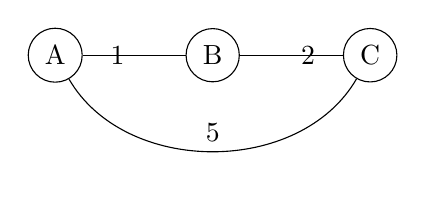
\begin{tikzpicture}
                    \node[shape=circle,draw=black] (A) at (0,0) {A};
                    \node[shape=circle,draw=black] (B) at (2,0) {B};
                    \node[shape=circle,draw=black] (C) at (4,0) {C};
                    
                    \path [-] (A) edge node[left] {1} (B);
                    \path [-] (B) edge node[right] {2} (C);
                    \path [-] (A) edge[bend right=60] node[above] {5} (C);
                    \end{tikzpicture}
               \end{center}

               
        
               Inicialmente, $d[A]=0$, $d[B]=\infty$, y $d[C]=\infty$. En la primera iteración, la distancia desde $A$ a $B$ se actualiza a $1$ y la distancia desde $A$ a $C$ se actualiza a $5$. En la segunda iteración, se actualiza la distancia desde $A$ a $C$ a través de $B$ a $3$.
            
               Aquí, la \textbf{subestructura óptima} se muestra por el hecho de que el camino más corto de $A$ a $C$ puede ser dividido en subcaminos más cortos de $A$ a $B$ y de $B$ a $C$. La solución al problema más grande (el camino más corto de $A$ a $C$) depende de la solución a los subproblemas más pequeños (los caminos más cortos de $A$ a $B$ y de $B$ a $C$).
            
               Los \textbf{subproblemas traslapados} se dan porque calculamos el camino más corto de $A$ a $B$ y de $B$ a $C$, y ambos subproblemas comparten el subproblema de calcular el camino más corto de $B$ a $C$.
            
                \item La recurrencia para el algoritmo Bellman-Ford se puede expresar como sigue:
            
               \[d[v] = \min(d[v], d[u] + w(u, v))\]
            
               donde $d[v]$ es la distancia más corta conocida desde $s$ a $v$, $d[u]$ es la distancia más corta conocida desde $s$ a $u$, y $w(u, v)$ es el peso de la arista de $u$ a $v$.
            
               Esta recurrencia se calcula para cada arista $(u, v)$ en cada iteración del algoritmo, actualizando $d[v]$ si se encuentra un camino más corto a través de $u$. Como resultado, después de $|V|-1$ iteraciones, $d[v]$ para todos los $v \in V$ será la distancia más corta desde $s$ a $v$, siempre que no existan ciclos de peso negativo.
            
        \end{itemize}

    \end{sol}
\end{problema}


%---------------------------
%\bibliographystyle{apa}
%\bibliography{referencias.bib}

\end{document}